\documentclass{article}

\usepackage{hyperref}
\usepackage{graphicx}
\usepackage{multirow}
\usepackage{subfig}
\usepackage{float}
\usepackage{longtable}
%\usepackage{blindtext}
\usepackage[margin=1.0in]{geometry}

\graphicspath{{./fig/}}

\begin{document}


\title{Physically Based Sound\\CIS 563}
\date{May 4, 2012}
\author{Jiali Sheng and Jordan Brindza}
\maketitle
  

\section{Introduction}

  For this project, we plan to physically generate sound for rigid body
  collisions. To simulate sound, we followed the implementation of the paper
  "Interactive Sound Synthesis for Large Scale Environments"~\cite{Raghuvanshi}. First, we
  reconstructed the objects in the scene as mass spring systems, and calculated
  the Gain matrix , and other coefficients as according to the paper. During
  run-time, we apply the force onto our mass-spring system to generate multiple
  signals that sum up to a sound wave. 

\section{Sound Modeling}

  We first looked at our input data. Our input is an XML file with information
  on how to generate a few supported primitives. With these primitives, we
  generated a mass-spring system based on our guess of how a mesh of the same
  primitive would look like. Figure~\ref{fig:cube_mesh} shows a simple example of a cube
  primitive. We store the data in an adjacency list. 

  \begin{figure}[H]
    \begin{center}
      \includegraphics[width=0.8\columnwidth]{cube_mesh_mesh_plot}
    \end{center} 
    \caption{Simple, example mesh for a cube with particles at each corner.}
    \label{fig:cube_mesh}
  \end{figure}

  Given our mass-spring system in the adjacency list, we then have to calculate
  the elastic force matrix (we'll call it the $K$-matrix). We assumed that all the
  springs in the mass spring system have the same $k$-constant. By Young's Modulus
  Theorem, this means we can factor the $k$-constant out when we first calculate
  the matrix. This $K$-matrix is a square matrix of size $3n$ by $3n$ -- $n$ is the
  number of particles in the system. For the $K$-matrix, for each spring (from mass
  $i$ to mass $j$), we will do $+1$ on cells  ($i$,$i$) and ($j$,$j$), and $-1$
  on cells ($i$,$j$), and ($j$,$i$), this is repeated for $2N$ and $3N$.
  Figure~\ref{fig:kmatrix} shows a visualization of our $K$-matrix for the cube. 

  \begin{figure}[H]
    \begin{center}
        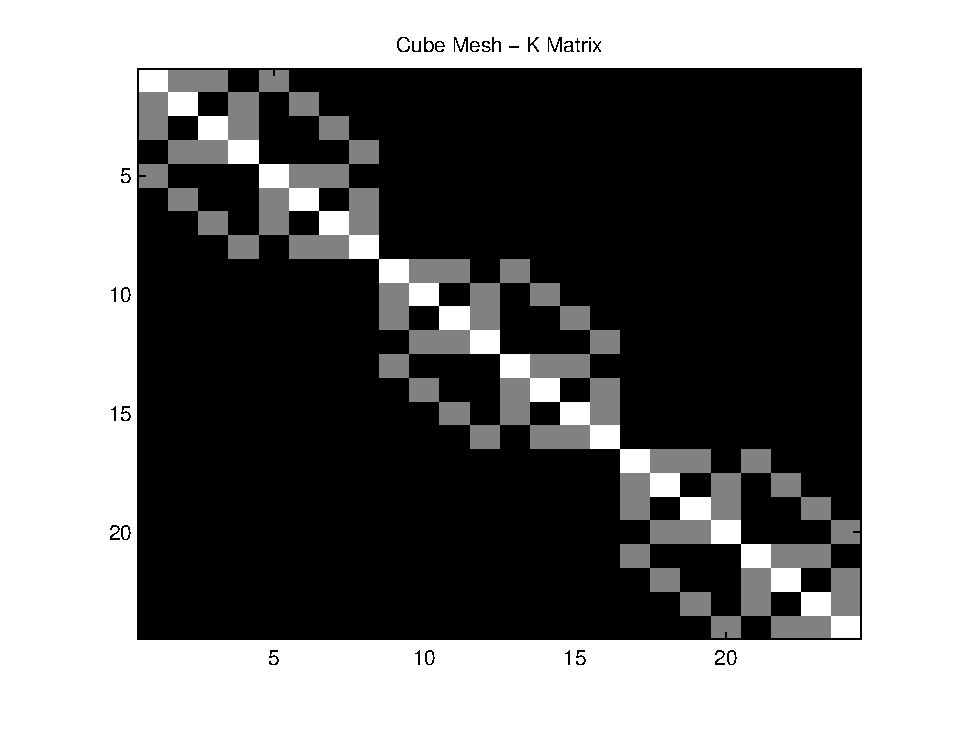
\includegraphics[width=0.8\columnwidth]{cube_mesh_Kmatrix} 
    \end{center} 
    \caption{Visualization of the full $K$ matrix for the simple cube mesh. The
              black cells are $0$, the gray cells have the value $-k$ and the white
              cells have the value $+2k$.}
    \label{fig:kmatrix}
  \end{figure}



  We then setup the equations of motion for the particle system as described in
  the paper. We assume that the displacement of the particles is small in order
  to use a linear approximation of the second order system:

  $$
    % system model ODE
    M\frac{d^2 r}{dt^2} + (\gamma M + \eta K) \frac{dr}{dt} + Kr = f
  $$

  Here $M$ represents the diagonal matrix of particle masses, $K$ is the force
  matrix described above and $r$ is the particles displacement. $\gamma$ and
  $\eta$ are free parameters representing the damping coefficients of the
  mass-spring system. In order to solve the equation we diagonalize $K$
  (utilizing the Eigen C++ library~\cite{Eigen}):

  $$
    % diagonalized K
    K = GDG^{-1}
  $$

  and substituting for $K$ in the original equation we get:

  $$
    % substituting for K
    \begin{array}{ccc}
      M\frac{d^2 r}{dt^2} + (\gamma M + \eta GDG^{-1}) \frac{dr}{dt} + GDG^{-1}r & = & f \\[11pt]
      G^{-1} M\frac{d^2 r}{dt^2} + (\gamma G^{-1} M + \eta DG^{-1}) \frac{dr}{dt} + DG^{-1}r & = & G^{-1} f \\[11pt]
      \textrm{$M$ is diagonal so } G^{-1}M = MG^{-1} & & \\[11pt]
      M G^{-1} \frac{d^2 r}{dt^2} + (\gamma M + \eta D)G^{-1} \frac{dr}{dt} + DG^{-1}r & = & G^{-1} f \\[11pt]
      \textrm{Using change of variables let } z = G^{-1} r & & \\[11pt]
      M \frac{d^2 z}{dt^2} + (\gamma M + \eta D) \frac{dz}{dt} + Dz & = & G^{-1} f \\[11pt]
    \end{array}
  $$

  Since $M$ and $D$ are diagonal matrices we end up with a set of $3n$ linearly
  independent equations in $z_i$, with each $z_i$ corresponding to the modes of
  the sound. The solution for each $z_i$ is then just the solution for a damped
  oscillator:

  $$
    % ode solution for damped oscillator 
    \begin{array}{ccc}
      z_{i}(t) & = & c_{i} e^{w_{i}^{+}t} + \bar{c}_{i} e^{w_{i}^{-}t} \\[11pt] 
      w_{i}^{\pm} & = & \frac{-(\gamma \lambda_{i} + \eta) \pm \sqrt{(\gamma \lambda_{i} + \eta)^2 - 4 \lambda_{i}}}{2}
    \end{array}
  $$

  where $\lambda_i$ is the $i$th eigenvalue of the $K$-matrix. The constants
  $c_i$ are initialized to zero and updated for a given collision impulse:

  $$
    % constants update from impulse
    c_{i} \gets c_{i} + \frac{g_{i}}{m_{i} (w_{i}^{+} - w_{i}^{-}) e^{w_{i}^{+} t_{0}}}
  $$

  The final response for each mode produced by the object is computed using the Euler's equation
  and the velocity of the modes:

  $$
    % derivative of z_i
    v_{i} = \frac{dz_{i}}{dt} = c_{i} w_{i}^{+} e^{w_{i}^{+}t} + \bar{c}_{i} w_{i}^{-} e^{w_{i}^{-}t}  
  $$

  Finally, the sound produced by the object is the summation of each individual
  mode which is played using the FMOD sound libraries~\cite{FMOD}.
  Figure~\ref{fig:mode_resp} shows graphs of the signals produced by striking
  the cube and sampling at different rates. 

  \begin{figure}[H]
    \begin{center}$
      \begin{tabular}{cc}
        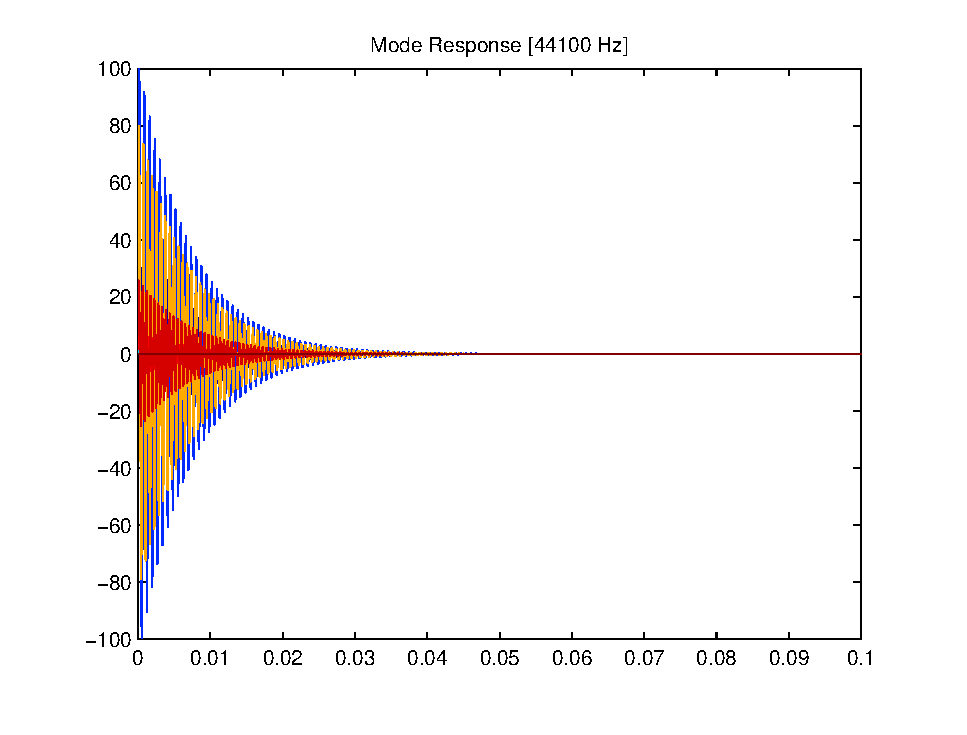
\includegraphics[width=0.5\columnwidth]{cube_mode_resp_44100hz}
        &
        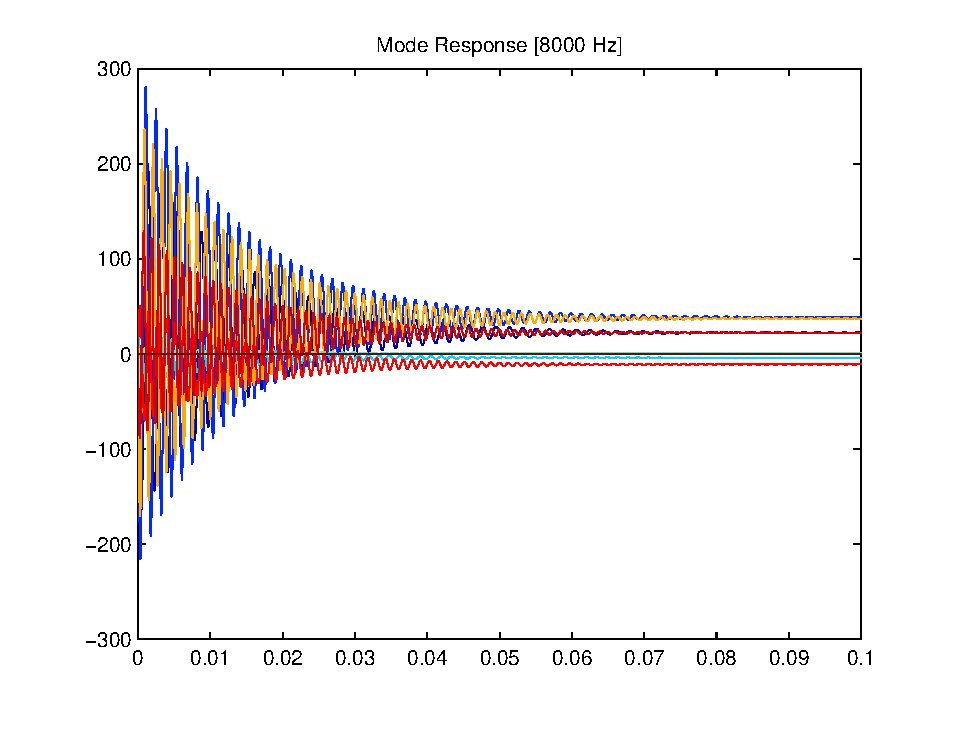
\includegraphics[width=0.5\columnwidth]{cube_mode_resp_8000hz} 
      \\
        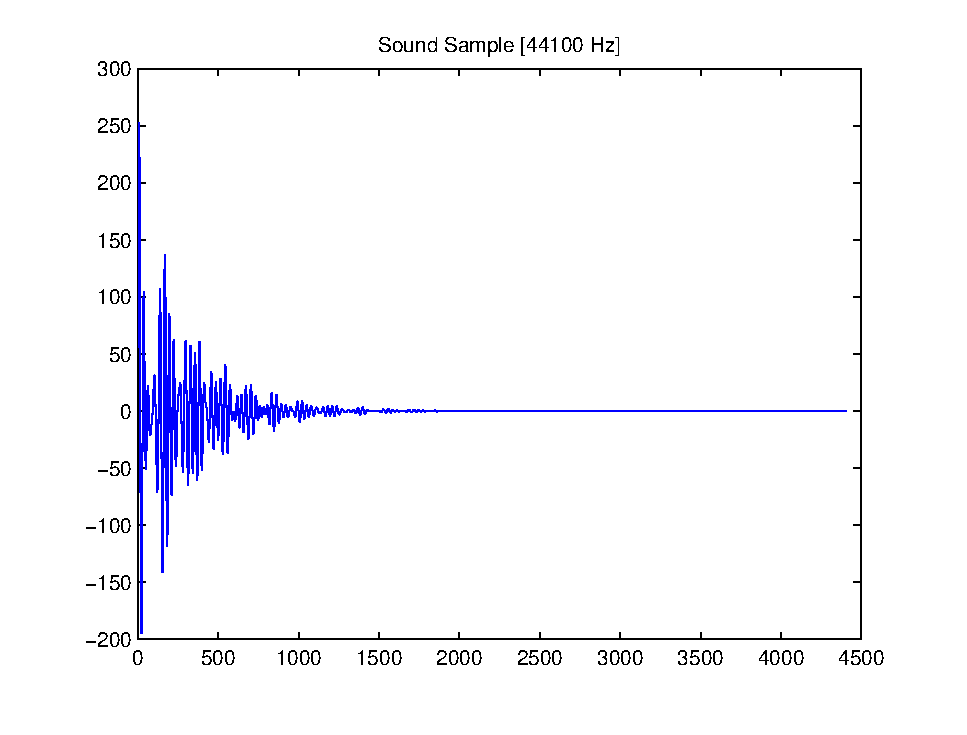
\includegraphics[width=0.5\columnwidth]{sound_sample_44100hz}
        &
        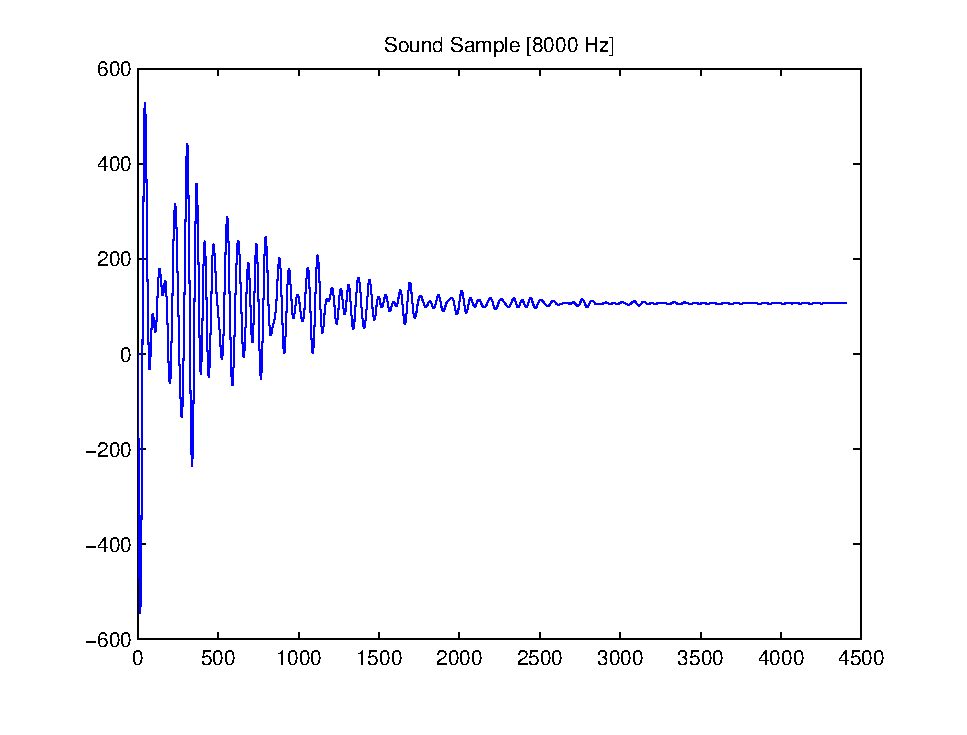
\includegraphics[width=0.5\columnwidth]{sound_sample_8000hz}
      \end{tabular}$
    \end{center}
    \caption{Plots of synthesized sound for a unit impulse on one of the cube
              vertices. The top row shows the individual mode responses (left was created
              at 44.1 kHz and the right at 8 kHz). The bottom row is the final sound
              sample of the summed mode responses (the left was sampled at 44.1
              kHz and the right at 8 kHz).}
    \label{fig:mode_resp}
  \end{figure}

\section{Results}

  Please check out our YouTube channel and blog for videos of the project
  results.

  \begin{itemize}
    \item YouTube: \url{http://www.youtube.com/watch?v=_wkh72SePL4}
    \item  Blog: \url{http://soundgen.tumblr.com}
  \end{itemize}

  % table example
  %\begin{center}
  %  \begin{tabular}{|c|c|c|c|}
  %    \hline
  %    Environment & Completion Time [s] & Max Position Error [m] & Max Orientation Error \\
  %    \hline
  %    1         & $85.40 $ &  $0.5220$ & $1.9745$ \\
  %    1         & $85.72 $ &  $0.3895$ & $0.1701$ \\
  %    7         & $120.52$ &  $0.9430$ & $0.5883$ \\
  %    7.2       & $120.82$ &  $1.2152$ & $1.9514$ \\
  %    \hline
  %  \end{tabular}
  %  \label{tab:myfirsttable}
  %\end{center}

  % grouped images example
  %\begin{figure}[H]
  %  \begin{center}$
  %    \begin{tabular}{cc}
  %      \includegraphics[width=0.5\columnwidth]{block_match_left_rgb}
  %      &
  %      \includegraphics[width=0.5\columnwidth]{block_match_left_block_seg} 
  %    \end{tabular}$
  %  \end{center}
  %  \caption{Example RGB image (left) and segmented regions (right).}
  %\end{figure}

  % single image example
  %\begin{figure}[H]
  %  \begin{center}
  %    \includegraphics[width=0.8\columnwidth]{block_match_stereo_corr}
  %  \end{center} 
  %  \caption{Example stereo correspondence.}
  %\end{figure}


\bibliography{report} \bibliographystyle{plain}

\end{document}

